\chapter{Experimentos}
\label{experimentos}
A lo largo de esta sección, se tratarán de forma detallada los distintos experimentos que se han realizado para este proyecto con el fin de 
poner en práctica los conocimientos obtenidos durante el proceso de investigación de la materia. Para cada experimento se planteará cuál es el 
objetivo a alcanzar y los posibles enfoques a aplicar para llegar a una solución, además de tratar los retos encontrados por el camino, los 
resultados del experimento y las lecciones que puedan ser aprendidas de este.

\section{Prueba de concepto Qiling}
\section{Fuzzing de un parser JSON}
\section{Identificación de vulnerabilidad real a través de fuzzing: Netgear R7000}
\subsection{Introducción al dispositivo}
El Netgear R7000, también conocido como Nighthawk AC1900 es un router WIFI ''inteligente'' lanzado al mercado originalmente en 2013 con una última
revisión del hardware en 2018 que sigue en venta actualmente. Este producto de la gama de routers premium de Netgear recibe actualizaciones periódicas
a día de hoy por parte del fabricante y se trata de una elección muy popular entre aquellos consumidores que buscan un router dual-band de altas prestaciones. 
\begin{figure}[H]
    \centering
    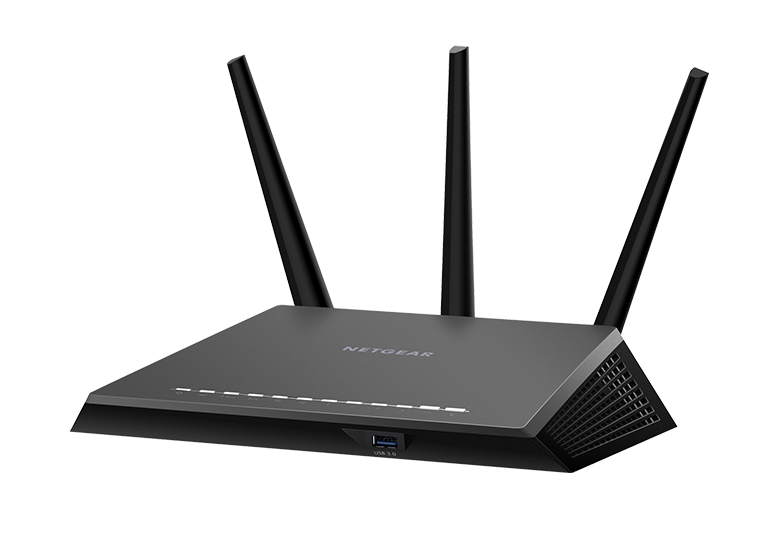
\includegraphics[scale=0.30]{r7000.png}
    \caption{Netgear R7000 (Nighthawk AC1900).}
    \label{fig:r7000}
\end{figure}

\subsection{Recopilación de información}
Consultando sus especificaciones técnicas principales 
encontramos que posee una CPU de 1GHz dual-core, 256MB de RAM, 128MB de memoria flash y soporte para dual-band de 2'4GHz a 600Mbps y de 5GHz a 
1300Mbps. Aunque estas especificaciones son interesantes a la hora de conocer las restricciones cómo de restringido en rendimiento es el dispositivo,
no son lo suficientemente detalladas como para aportarnos información clave que necesitamos conocer para aplicar emulación sobre el dispositivo.
Principalmente, desconocemos el procesador que está siendo utilizado y su arquitectura, ya que el fabricante no proporciona dicha información.
Cuando nos encontramos en esta situación en la que deseamos conocer información más detallada sobre los componentes internos de un dispositivo, 
una posible solución es consultar su informe de aceptación para la certificación del FCC [TBD REFERENCIA] en la base de datos \hyperlink{fccid.io}{fccid.io}.
El FCC es un organismo de certificación encargado de evaluar todo producto que vaya a ser comercializado en los Estados Unidos que emita 
radiofrecuencias con el fin de asegurar que dichos dispositivos no produzcan interferencias dañinas que pudieran afectar al correcto
funcionamiento de otros dispositivos como equipamiento médico, aeronáutico o sistemas de telecomunicaciones.\bigskip

Accediendo a la base de datos podemos encontrar información de los reportes que se han ido realizando sobre las distintas iteraciones del producto,
concretamente, el reporte de mayor interés para nuestra tarea es el titulado ''Internal Photos'' publicado para la revisión lanzada en 2018\cite{netgearFCCid}.
Buscando lo que pudiera ser la CPU principal nos llaman la atención dos chips mostrados en el informe. El primero (figura \ref{fig:r7000transceptor}), al 
consultar la ficha técnica del BCM4360 descubrimos que se trata de un transceptor WIFI del fabricante Broadcom, por lo tanto no es lo que tratamos de 
encontrar. Respecto al segundo chip (figura \ref{fig:r7000cpu}), consultando las especificaciones presentes en la ficha técnica del Netgear R7000 
(tabla \ref{table:r7000}) proporcionada por OpenWRT podemos ver que se trata de un System on a Chip (SoC) WIFI lanzado al mercado en 2013\cite{broadcomSOCs} 
que en su interior contiene un procesador dual core ARM Cortex A9 de 32 bits.

\begin{figure}[H]
    \centering
    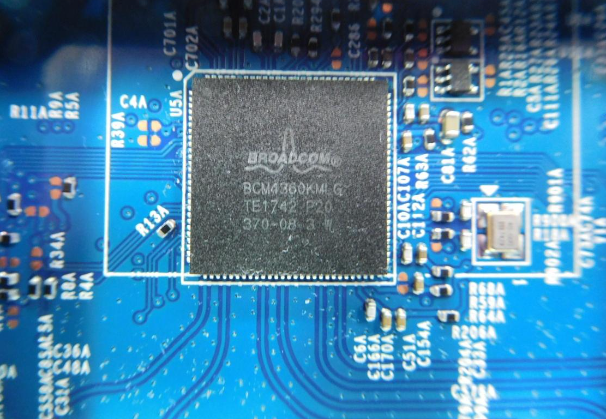
\includegraphics[scale=0.45]{r7000transceptor.png}
    \caption{Broadcom BCM4360 en el interior del Netgear R7000.\cite{netgearFCCid}}
    \label{fig:r7000transceptor}
\end{figure}

\begin{figure}[H]
    \centering
    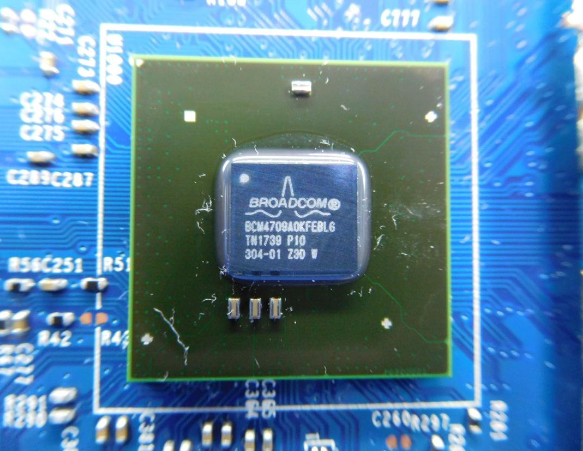
\includegraphics[scale=0.59]{r7000cpu.png}
    \caption{Broadcom BCM47 en el interior del Netgear R7000.\cite{netgearFCCid}}
    \label{fig:r7000cpu}
\end{figure}

\begin{table}[H]
    \centering
    \begin{tabular}{ |l|m{20em}| }
    \hline
    FCC ID                      & PY313200233                      \\\hline
    Industry Canada ID          & 4054A-13200233                   \\\hline
    Voltaje                     & 12 VDC, 3.5 A                    \\\hline
    CPU/SoC                     & Broadcom BCM4709A0 @1 GHz        \\\hline
    Arquitectura CPU            & ARM Cortex A9 (2 cores)          \\\hline
    Flash / RAM                 & 128 MiB / 256 MiB                \\\hline
    Chip WI1 \& WI2             & Broadcom BCM4360                 \\\hline
    Protocolos WI1 \& WI2       & an+ac / bgn                      \\\hline
    Configuración MIMO wireless & 3x3:3                            \\\hline
    Conector de antena          & U.FL, RP-SMA                     \\\hline
    Switch \& Ethernet          & Broadcom BCM4709A0               \\\hline
    Puertos WAN/LAN             & 1 / 4 (up to 1 Gb/s)             \\\hline
    Puertos USB                 & 1x USB 3.0, 1x USB 2.0           \\\hline
    Puerto serie                & 4-pin header, internal, 3.3V TTL \\\hline
    \end{tabular}
    \caption{Especificaciones del Netgear R7000.\cite{r7000datasheet}}
    \label{table:r7000}
\end{table}

Aunque Broadcom no proporciona una datasheet con las especificaciones del SoC, 
si que podemos consultar información más detallada sobre el Cortex A9 a través de la documentación oficial de ARM\cite{cortexA9}. Gracias a esto podemos 
conocer detalles como información sobre la Memory Management Unit (MMU) que utiliza la CPU. Esta información es de gran importancia ya que como explicaban
Muench et al.\cite{Muench2018}, la presencia de una MMU en un dispositivo empotrado puede alterar drásticamente el comportamiento de este ante corrupciones de 
memoria. Un dispositivo sin MMU puede no detectar fallas de memoria y seguir funcionando en un estado indefinido mientras que uno con MMU provoca un 
crash al detectar corrupción de memoria o la realización de alguna operación ilegal. Según la documentación oficial de la CPU, el procesador utiliza la MMU 
diseñada para la arquitectura Armv7, por lo que podemos deducir que un crash que encontremos aplicando fuzzing al firmware mediante emulación, podrá ser replicado
en el dispositivo real.

\subsection{Obtención del firmware}
Una vez hemos recopilado información sobre el objeto de estudio, necesitaremos conseguir el firmware del dispositivo para proceder a su análisis y posterior 
emulación. A la hora de conseguir el firmware de un dispositivo IoT podemos enfrentarnos a una serie de retos dependiendo de cómo el fabricante distribuya
las imágenes del firmware. Podemos categorizarlos de la siguiente mantera:
\begin{itemize}
    \item \textbf{Medio de distribución}: En el mejor de los casos, el fabricante provee un enlace de descarga del firmware a través de su portal de soporte oficial. Aunque
    este suele ser el caso para dispositivos como routers o cámaras IP, no es común en otros dispositivos aún más limitados como bombillas inteligentes o asistentes de voz.
    También hay fabricantes que con el objetivo de intentar evitar que usuarios puedan aplicar técnicas de ingeniería inversa sobre los paquetes de actualización, integran 
    todo el proceso de actualización a través de una app móvil o desde el propio dispositivo. Ante esto, es posible hacer uso de iptables para redirigir el tráfico
    de la aplicación o del dispositivo e intentar interceptar las peticiones al servidor de descargas de firmware. Por último, existe la posibilidad de que el fabricante no 
    haya provisto al dispositivo de un mecanismo de actualización para el usuario. Como último recurso, sería posible desmontar el dispositivo e intentar extraer el firmware 
    a través de la interfaz JTAG o leyendo los contenidos de la memoria FLASH utilizando un programador flash (figura \ref{fig:programador}).
    \begin{figure}[H]
        \centering
        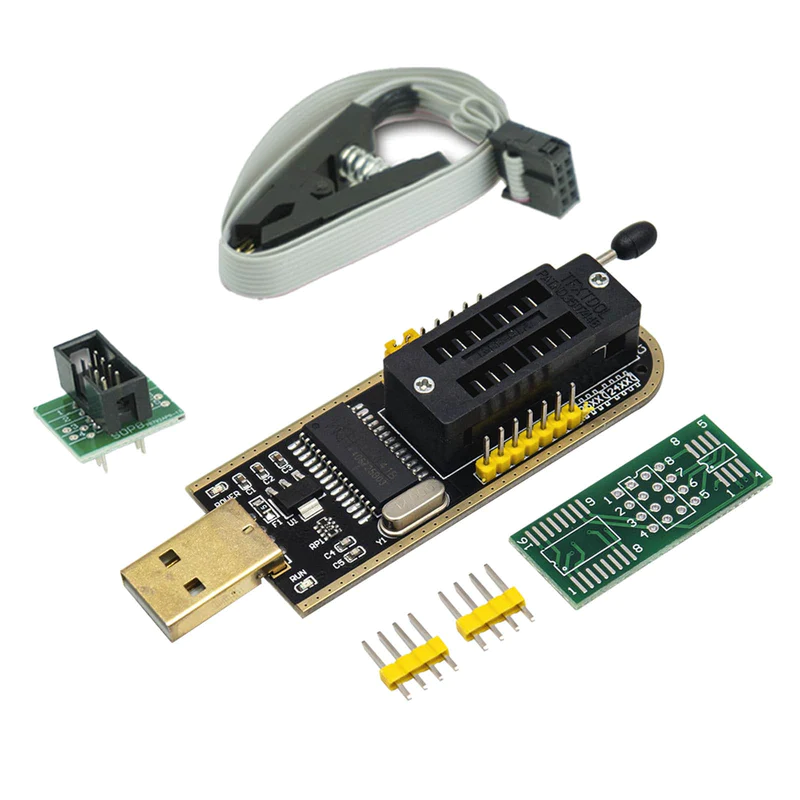
\includegraphics[scale=0.35]{programmer.png}
        \caption{Programador flash CH341A genérico.}
        \label{fig:programador}
    \end{figure}
    \item \textbf{Cifrado}: Además de no proporcionar un portal de descargas de firmware, los fabricantes también suelen cifrar sus paquetes de actualización para dificultar las 
    tareas de análisis e ingeniería inversa. Dicho firmware es posteriormente descifrado por la rutina de actualización del dispositivo. Cuando se da este caso desgraciadamente 
    solo quedan dos opciones, o extraer el firmware del mismo dispositivo como se ha comentado en el punto anterior o intentar obtener la versión del firmware previa a que el 
    fabricante implementara el cifrado en las actualizaciones y aplicar ingeniería inversa sobre la rutina de descifrado del firmware para llevar a cabo nuestra propia implementación. 
    \item \textbf{Formato}: Es bastante común para los fabricantes distribuir sus paquetes de firmware en formatos propietarios difíciles de tratar sin software especializado. 
    Binwalk\cite{binwalk} es una herramienta que puede ayudar con el análisis y desenpaquetado de imágenes firmware en binarios de los cuales se desconoce su estructura. El uso de esta herramienta
    será tratado a continuación. También es posible que se den casos en los que binwalk no sea capaz de identificar o extraer correctamente el contenido de la imagen firmware, 
    teniendo que recurrir al diseño de herramientas específicas para el firmware con el que se está trabajando, identificando los offsets a partir de dónde empiezan los distintos 
    componentes de este y extrayéndolos manualmente con herramientas como dd de las coreutils de GNU.
\end{itemize}

Para el Netgear R7000, es posible obtener el firmware a través de su \href{https://www.netgear.es/support/product/r7000.aspx#download}{portal oficial de soporte}. Una vez 
descargado el paquete de firmware versión 1.0.11.128, procedemos a su análisis con la herramienta Binwalk. El primer paso es comprobar si el binario se encuentra cifrado mediante 
la comprobación de su entropía. La entropía del binario es un valor que representa el nivel de aleatoriedad entre los bytes del fichero y un valor alto constante
en todo el binario es un fuerte indicativo de que o su contenido ha sido comprimido o que este ha sido cifrado. Para consultar la entropía representada en una gráfica usamos Binwalk con la siguiente orden. 
\begin{lstlisting}[language=bash]
  $ binwalk -E R7000-V1.0.11.128_10.2.112.chk
\end{lstlisting}

Como podemos apreciar en la figura \ref{fig:binwalkEnt}, Binwalk reporta una entropía considerablemente alta para el firmware. Para comprobar si estamos
ante un firmware cifrado intentamos identificar el contenido de este usando la flag ''-e'' en lugar de ''-E''. Al hacerlo, Binwalk es capaz de detectar 
la presencia de tres elementos dentro del firmware (\ref{fig:binwalkExt}), una primera entrada de nombre ''TRX firmware header'' que contiene metadatos
del firmware en formato TRX como un magic number, la versión de TRX en uso, longitud del header o un checksum CRC32 para comprobar la integridad del paquete. Sería posible
identificar qué información corresponde a cada campo consultando la documentación sobre el formato TRX\cite{firmwareFormat}, pero Binwalk ya hace este trabajo 
por nosotros. Además, Binwalk nos indica que estamos ante un firmware basado en Linux. A continuación identifica una sección de datos comprimidos usando LZMA, un algoritmo
de compresión sin pérdidas usado en este caso para comprimir la imagen del Kernel de Linux. Por último, tenemos el sistema de archivos del dispositivo en formato
SquashFS, un sistema de archivos de solo lectura utilizado en dispositivos de recursos limitados por sus capacidades de compresión. Tras la extracción, tenemos acceso 
al contenido del sistema de archivos además de la imagen del Kernel.

\begin{figure}[H]
    \centering
    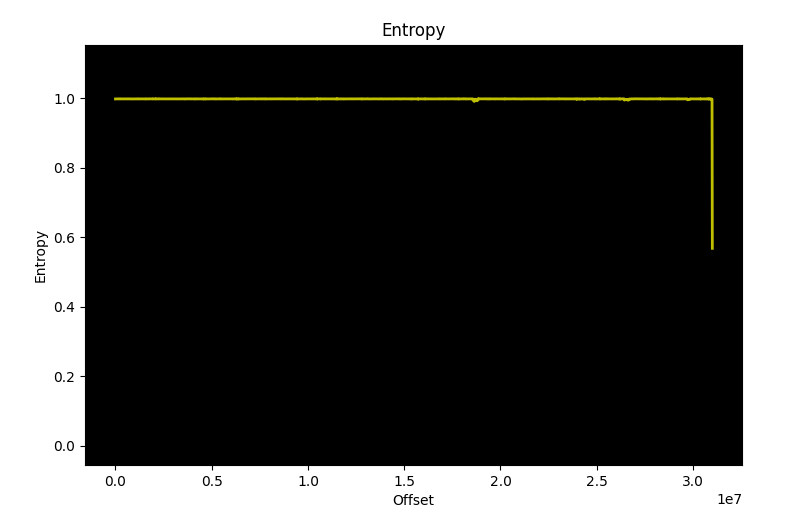
\includegraphics[scale=0.35]{r7000entropy.png}
    \caption{Gráfica de la entropía de la imagen firmware del Netgear R7000 generada por Binwalk.}
    \label{fig:binwalkEnt}
\end{figure}

\begin{figure}[H]
    \centering
    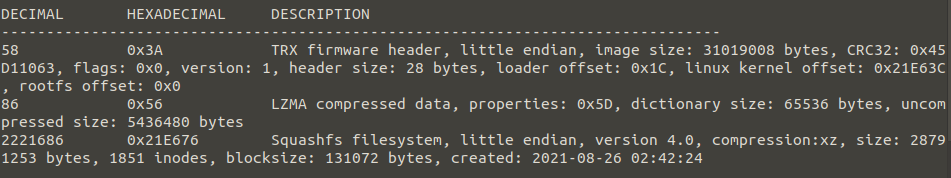
\includegraphics[scale=0.36]{r7000extraction.png}
    \caption{Extracción firmware Netgear R7000 usando Binwalk-}
    \label{fig:binwalkExt}
\end{figure}





\subsection{Introducción al experimento}
\subsection{Realización del experimento}
